 \begin{center}\begin{large} Homework Problems 4 (Functions of Several Variables; Probability) \end{large}\end{center}
 \bigskip






\begin{problem}%[\textbf{optional, not graded}]
Match the graphs 1-4 to functions i-iv: 
\begin{center}
\\~\\
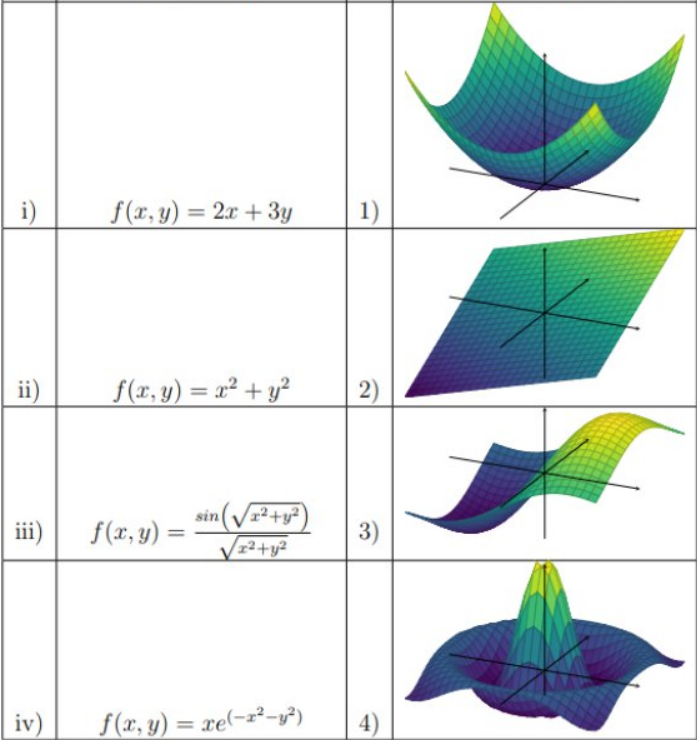
\includegraphics[width=0.6\linewidth]{figs/f(x,y) functions.png}
\\~\\
\end{center}
\end{problem}

\medskip




% \begin{problem}[2 points]
% Find the gradient and the Hessian of the following functions: 
%     \begin{enumerate}
%     \item[a) ] $f(x,y) = 6x-y^2$,
%     \item[b) ] $f(x,y) = x^2 y^2 - 4xy + 1$,
%     \item[c) ] $f(x,y) = \dfrac{\cos x}{y}$,
%     \item[d) ] $f(x,y) = \ln(xy)$,
%     \item[e) ] $f(x,y,z)=x^5 - 4yz^2$,
%     \item[f) ] $f(x,y,z)=xyz$.
%     \end{enumerate}
% \end{problem}
% \bigskip




\begin{problem}
Find the partial derivatives:
\begin{enumerate}
        \item[a) ] $f(x,y)=3x-2y^2$
        \item[b) ] $f(x,y)=y^7-2x^3+x^2$
        \item[c) ] $f(x,y)=\sin{xy}$
        \item[d) ] $f(x,y)=x \cdot \ln y+\dfrac{x}{y}$
    \end{enumerate}
\end{problem}
\medskip 


\begin{problem}
Compute the directional derivative  at the point $(-1,-1)$ along the vector $\vv=[0.6,\,0.8]$:
\begin{enumerate}
    \item[a) ] $f(x,y) = 3xy$
    % \item[b) ] $f(x,y) = 1-x^2$
    \item[b) ] $f(x,y) = e^{x-y}$
    \end{enumerate}
\end{problem}


\medskip 


\begin{problem}
In Lake Sevan, the depth of water at the point with coordinates
$(x,y)$ is 
\[xy^{2}-6x^{2}-3y^{2}\]
meters. As the captain of the ship "Noratus" (which is currently at the point $(5, 3)$) wants to get to a deeper part of the lake,  his first mate suggests to sail north, while the second mate recommends sailing south. Which mate should the captain listen to?
\end{problem}


% \begin{problem}
% Calculate the directional derivative:
% \begin{enumerate}
%         \item[a) ] $f(x, y) = (x-y)^2$ at the point $(1, 2)$ in the direction of $\dfrac{\vv}{\|\vv\|},\,\vv = (3,-4)$,
%         \item[b) ] $f(x, y) = x \log y + (1-x) \log (1-y)$ at the point $(\pi, 0)$ in the direction of $\dfrac{\vv}{\|\vv\|},\,\vv = (1,1)$.
%     \end{enumerate}

% {\small Note: $\log x=\ln x$.}
    
% \end{problem}

\medskip


\begin{problem}
Does  the following function have local extrema? If so, find them:
\begin{enumerate}
    \item[a) ] $f(x,y) = 3xy$
    \item[b) ] $f(x,y) = x^2-xy$
    \item[c) ] $f(x, y) = 2x^2 - x^3 - y^2$
    \end{enumerate}
You can  plot the graph  or use the $D$ on the last slide.
\end{problem}
\medskip



\begin{problem}[\textbf{additional}]
You have $12$ square meters of cardboard (as well as scissors, and glue) and this time you want to make a topless box (i.e. no upper side) like this:
\begin{center}
\\~\\
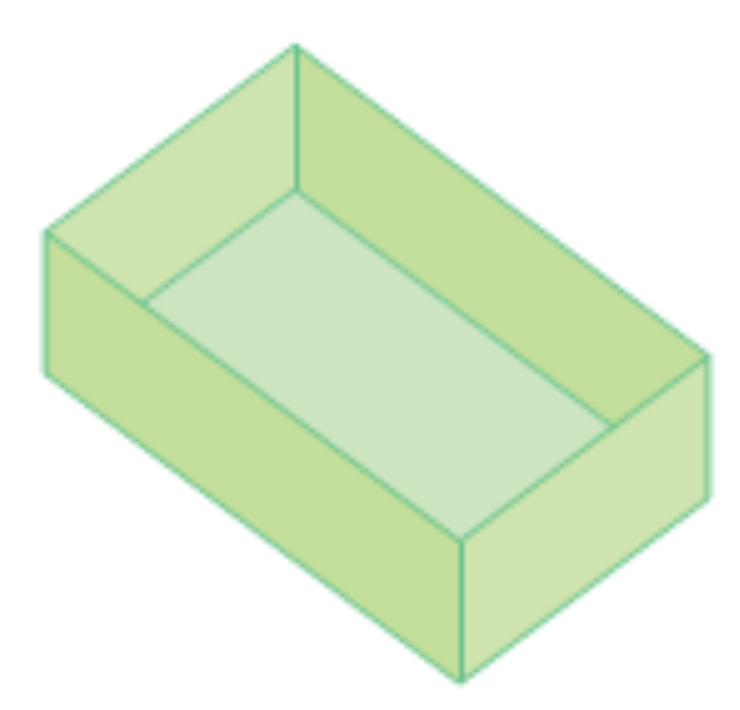
\includegraphics[width=0.3\linewidth]{figs/topless-box.png}
\\~\\
\end{center}
What is the maximum volume your box can have?



\smallskip 

{\small \textit{Hint:  This time we have no squares, so you can denote its height, length and width by $x$, $y$ and $z$. Can you express $z$ by $x$ and $y$? Can you then express the volume by $x$ and $y$? How do we find the maximum value of a function of two variables?}
    }
\end{problem}


\medskip
        

\begin{problem}[\textbf{additional}]
There are a couple of ways to make one new function from two given functions. One of them is \textit{convolution} which is an  important technique in ML.

For any two functions $f$ and $g$,  their convolution is a new function $f*g$, which is defined by the formula:
\[
(f*g)(x) = \int_{-1}^1 f(y)g(x-y) \, dy \qquad \text{(where $x$ is fixed)}
\]
Given $f(x)=x^2$ and \[g(x) = \begin{cases}
    1 & \text{if } x>0\\
    0 & \text{if } x \le 0
\end{cases}\]
find the value of $f*g$ at the point $x=0$.


\smallskip 

{\small \textit{Hint:  Plug in the formula for $g$, then divide $[-1,1]$ into two parts where $g=0$ and where $g=1$.}
    }
\end{problem}

\medskip



\begin{problem}
Suppose we roll two fair dice. What is the probability of getting
\begin{enumerate}
    \item[a) ] $2$ on each of them,
    \item[b) ] at least one $1$,
    \item[c) ] exactly one $1$,
    \item[d) ] one $1$ and one $4$,
    \item[e) ] $1$ on the first die and $4$ on the second die?
\end{enumerate}
\end{problem}
\medskip

\begin{problem}
There are $2$ red, $5$ blue and $6$ yellow pencils in the box. We take two of them out randomly. What is the probability that both of them are
\begin{enumerate}
    \item[a) ] red,
    \item[b) ] of the same color,
    \item[c) ] of different colors,
    \item[d) ] not yellow,
    \item[e) ] not green.
\end{enumerate}
\end{problem}
% \bigskip

\medskip

\begin{problem}
     \\~\\
\begin{center}
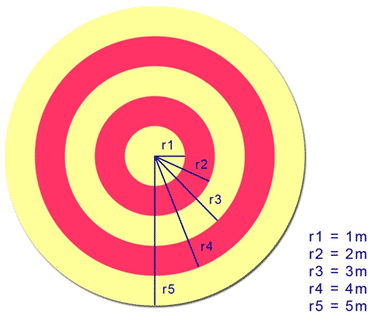
\includegraphics[width=0.5\linewidth]{figs/prob1.png}
\end{center}
\\~\\
Assume that any thrown dart will land somewhere within the circular area. The radius of circle $1$ (the inner-most yellow circle) is $1$ meter. Each radius thereafter increases by $1$ m, as shown. We throw a dart randomly. Find the probability that the circle it lands on
\begin{enumerate}
    \item[a) ] is the circle $1$,
    \item[b) ] is a red circle,
    \item[c) ] is a yellow circle.
    
\end{enumerate}
\end{problem}


\medskip


\begin{problem}
A fair coin is tossed 5 times. What is the probability of getting an odd number of heads?
\end{problem}

\medskip



        
\begin{problem}
Two fair dice are rolled. What is the probability of getting $1$ on at least one of them, given that we know their sum is even?
\end{problem}
\medskip

\begin{problem}[\textbf{additional}]
$3$ cards are drawn from a deck of $52$ cards. What is the probability that the first two cards are queens, and the third one is diamonds {\color{red}$\blacklozenge$}?
\end{problem}

\medskip 



\begin{problem}[\textbf{additional}]
There are $15$ books on a bookshelf, $5$ in Armenian, $10$ in French. Ruben cannot read French. If he randomly takes $3$ books, what is the probability that he can read at least one of them?
\end{problem}



% this one is stolen from Tarkhanyan
% 
% 
% 4 - Spam emails 
% \begin{problem} (Spam emails)
%         A spam filter tags emails as spam or not spam. Based on historical data:
%     \begin{itemize}
%         \item 80\% of spam emails contain the word "lottery."
%         \item 30\% of non-spam emails contain the word "lottery."
%         \item 40\% of emails are spam.
%     \end{itemize}
    
%     What is the probability that an email is spam given it contains the word "lottery"?
% \end{problem}
% 
% also, check my old practicals